\chapter{Project Deliverable - OpenStack REST Client Description}
\centerline{\rule{149mm}{.02in}}
\vspace{2cm}

\section{Introduction}
This appendix aims to give an introduction to the delivered code project called \textit{FYPRestExperiments}. \\
Firstly it will cover how the project is built, which technologies are used, and then will explain the design of the code itself, and in doing so describe how it can be re-used. 


\section{Project Build}

\subsection{Java}
The project uses Java 7\cite{java7}, and is therefore reliant on this version of Java to execute. Due to this, code being developed for this must be written using a Java-compatible technology, such as Java itself or another Java Virtual Machine language like Scala. Similarly, the Java 7 Runtime Environment must be installed in order to execute this application. 

\subsection{Maven}
In order to manage dependencies of the project, such as the Spring Framework\cite{springframework} or Apache's Log4J\cite{log4j} library, the dependency management tool Maven\cite{maven} was used. This tool manages the resolution of dependencies at build, compile or run-time, and simplifies the java build process. \\
Dependencies are stored in XML file in the \textit{pom.xml} file, which defines which software projects will be needed by the current project, including version details. From this, Maven automatically downloads the uses the correct version of the dependency. \\
To use this code for development, for example, using the Eclipse IDE\cite{eclipseide}, as I did in this project, a plugin for maven must be installed, but after this point, the project with dependencies will be built automatically as long as the \textit{pom.xml} file is present. Alternatively, maven can build the project from the command line; more information can be found at the Maven website. \\

By far the simplest way to execute this project is directly from the compiled classes in the main project directory \url{fyprestexperiments}. This can be performed with the \textit{mvn exec:java} command. Arguments can also be passed like so: \textit{mvn exec:java -Dexec.mainClass="fyp.main.ExperimentExecutor" -Dexec.args="test.xml another.xml"} Please ensure you give addresses of xml files relative to the classpath. 

An example of how to run this using maven on the command line is shown below: 

\begin{figure}[H]
\centering
\fbox{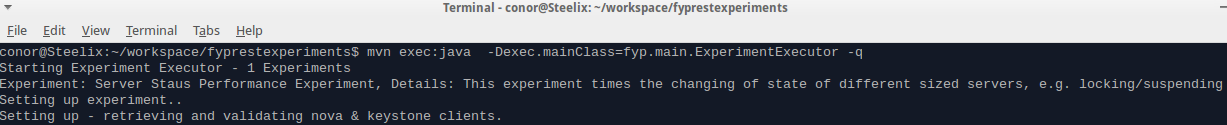
\includegraphics[scale=0.5]{mavenexec}}
\caption{Executing the project with maven on the command line}
\end{figure} 

\section{Project Design}
\subsection{Spring}
The use of Spring has been described briefly in the warm up exercises Appendix (D). The main uses of Spring have been: 
\begin{itemize}
\item Dependency Injection through Java Bean Config
\item Rest Template 
\end{itemize}

The idea behind using Springs JavaBean definition functionality was to allow other users to create their own XML files with their own OpenStack configuration and experiments to execute, meaning that the experiment framework and clients could be easily configured to work anywhere. \\

This project will take any number of arguments representing XML files, and will work as long as beans representing the following are available to the main class, (bean name - class):
\begin{itemize}
\item openstackConfigBean - fyp.config.OpenStackConfig
\item experiments - java.util.ArrayList<fyp.experiments.Experiment>
\end{itemize}

examples of each of these being implemented can be found in \url{fyprestexperiments/src/main/java/fyp/beans/Beans.xml} and \url{fyprestexperiments/src/main/java/fyp/beans/Experiments.xml} respectively. \\
As long as these beans are satisfied, the following automatic configuration takes place, thanks to Spring:
\begin{itemize}
\item Each subclass of OpenstackRestClient has access to the openstack config, so it knows where to send requests. 
\item Each subclass of Experiment has access to the config too, so it can pass information on where necessary.  
\item The experiment Executor knows which subclasses of Experiment to run, and has an instance of each one to execute. 
\end{itemize}

In this way, we have a very smooth execution process without any additional configuration. \\

The \textit{RestTemplate}\cite{resttemplate} class provided by Spring is a useful way of sending requests to a remote URL, using isntances of \textit{HTTPEntity}\cite{httpentity}. The biggest advantage of this is the ability to add a custom java object-JSON converter, in this case, Jackson\cite{jackson}. This meant all message translation was implicit and automatic, through creating classes to hold message data such as the \textit{fyp.nova.data.Server} class and specifying this class in the request. This can be seen in any of the client implementation classes.

\subsection{REST Clients}

The rest clients are very straightforward. They all subclass the \textit{OpenstackRestClient} class, which gives them access to the OpenStack configuration details such as login details and endpoints, and for each different type of client there is an interface specifying it's functionality. The class diagram shown in appendix D illustrates this well:

\begin{figure}[ht]
\centering
\fbox{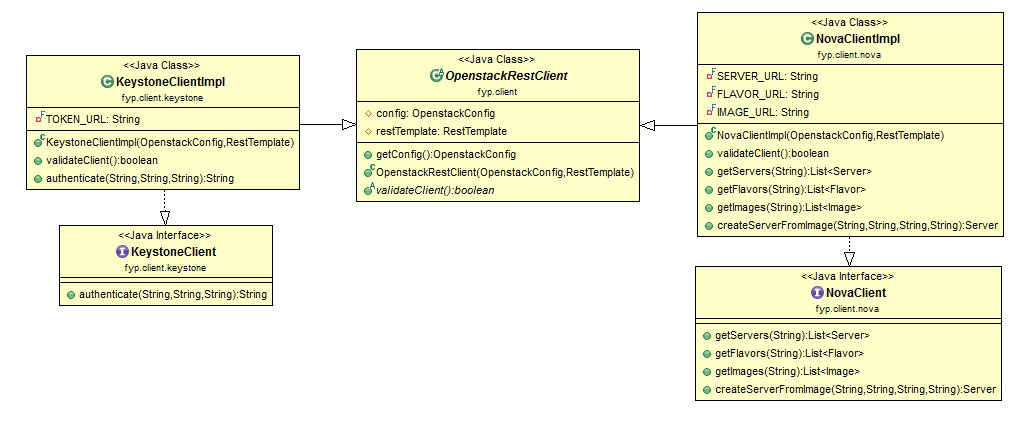
\includegraphics[scale=0.35]{clientclassdiagram}}
\caption{Class Diagram for Openstack clients} 
\end{figure}

These are all implemented to use the aforementioned RestTemplate to send requests based on the information from config and from which interface method is called by an experiment or other client.  \\
The only other piece of configuration concerns the creation of classes to hold request and response information. These can be found in the *.request and *.response packages/directories, and simply allow the jackson JSON converter to match the request or response body to an object. 

\subsection{Experiments}

Experiments were similarly explained in Appendix D. The idea behind writing experiments is to subclass the \textit{fyp.experiments.Experiment} class, providing config automatically, and a number of methods providing the structure of the experiment, such as \textit{setUp}, \textit{execute} and \textit{tearDown}. These methods are automatically called by the main class of this project, \textit{fyp.main.ExperimentExecutor}, and are called for every class defined in the Experiments config bean. 
This class diagram, again from the previous appendix, illustrates this architecture: 
\begin{figure}[ht]
\centering
\fbox{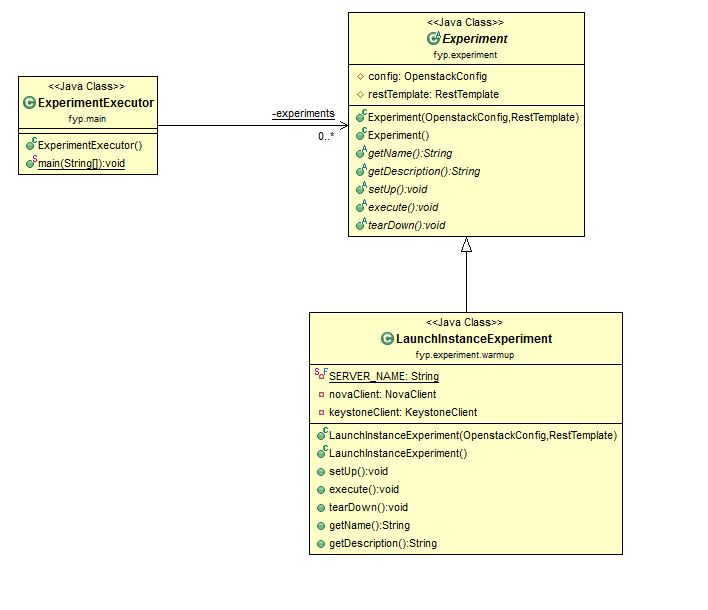
\includegraphics[scale=0.35]{experimentclassdiagram}}
\caption{Class Diagram for Experiment execution} 
\end{figure}

Practically, this means that to create a new experiment to work with this framework, all one needs to do is subclass \textit{Experiment}. 


\subsection{Utilities}

A small number of utilities were added to the project under the \textit{fyp.utils} package, usually to make up for shortcomings of the OpenStack rest apis. These are intended to be used by experiments for convenience, and are designed using static classes. \\

\section{Delivered Items}
The rest client project has delivered the following components: 
\begin{itemize}
\item Source code for a Maven Java project, found under \url{fypexperiments/src/} directory.
\item Compiled source code for execution with Maven \url{fyprestexperiments/target/}
\item A built, executable Jar file containing project code, \url{fypexperiments/target/openstackrestclient-0.0.1-SNAPSHOT.jar}
\item Example Spring Bean config files for reusability, found at \url{fyprestexperiments/src/main/java/fyp/beans/} directory.
\item A number of example experiments to execute or use as a guide found at \url{/home/conor/workspace/fyprestexperiments/src/main/java/fyp/experiment/}
directory.
\item A number of utilities which aid in using the provided rest client interfaces. Utilities: \url{fyprestexperiments/src/main/java/fyp/utils/} interfaces (with implementations): \url{fyprestexperiments/src/main/java/fyp/client/} 
\item logs of each experiment executed, found at \url{fyprestexperiments/logs} directory.
\end{itemize}



